\section{Project Proposal}
Initially, we planned to write a business plan to commercialise our product. However, after some brainstorming, we realised that the market that we could aim at effectively consists of secondary schools and sixth-forms. In addition, a business plan would require a well-defined aim and source of profit. It is unlikely that we could make a significant amount of profit by solely selling our product to schools. The need of this product on its own is insignificant, however, there are great public engagement opportunities that it offers. To find the silver lining between commercialisation and public engagement we have come up with a new idea. Instead of a business plan, we have written a business proposal aimed at STFC’s Public Engagement Sparks Award. This award would enable us to get funding and it would also help to reach and visit schools, given the resources of STFC. We believe that it is a strong and realistic plan and that it would genuinely motivate students to study STEM subjects.  

\subsection{Aims}

Our project aims to inspire the next generation of physicists and, in particular, secondary school students in the United Kingdom. We hope that students will form a more positive attitude towards STEM subjects. More precisely, our aim is to help students get a unique insight into quantum mechanics, therefore making the subject much more exciting and intuitive. We will achieve this by providing equipment with which the visualisation of complex quantum mechanical phenomena is made possible on a macroscopic level.

As part of our third year group project at University College London, we have assembled an apparatus with which the visualisation of quantum mechanical effects is possible. This consists of a woofer, on which a petri dish containing washing liquid is placed. The woofer drives the air under the petri dish which makes the surface of the oil vibrate too. With careful calibration of this apparatus, it is possible to make droplets, which vibrate above the immediate surface. A high-resolution photo of a bouncing droplet can be seen in Figure 1. These oil droplets behave exactly how the pilot-wave theory predicts how quantum particles should behave. Pilot-wave theory explains the behaviour of quantum particles ingeniously: it suggests that they consist of the particle itself and its pilot wave. When we see particle-like effects, we see the particle interacting, and when we see wave phenomena, the pilot wave is interacting with its own reflections. This can be imagined just like the particle and its wave in Figure \ref{fig:droplet_STFC_report}. Numerous quantum mechanical phenomena can be demonstrated and visualised using this apparatus, including the double-slit experiment or even a molecule-like structure of two particles. Simulations were also made as part of this project, to see how well prediction and experimentation agree in this case.  

\begin{center}
\begin{figure}[htb]
\centering
    
\includegraphics[width=8.996cm,height=5.997cm]{education/STFCproposal/Droplet_STFC.jpg}
    \caption{An image of a bouncing droplet captured mid-oscillation.}
    \label{fig:droplet_STFC_report}
\end{figure} 
\end{center}

In the public's view, quantum physics is a mysterious and unpredictable world. This apparatus provides an excellent opportunity to alter their perception and increase public engagement with quantum mechanics. Not only does it show numerous aspects of quantum mechanics, but also it helps make it seem less distant to people. It shows young students that, using the power of science, even such a strange world can be understood and manipulated.

Investigation of quantum phenomena is a significant proportion of today's physics research. To make students more familiar with quantum mechanics is essential to maintain, or even raise, the number of students choosing a science-related career.

Our eventual goal is to develop a compact product, with which bouncing oil droplets can be made, and to present it in schools. Potentially, depending on the demand, the apparatus can be manufactured and given or sold to schools, to enable them to conduct their own experiments in order to encourage their pupils' curiosity. 

\subsection{Objectives}

We have three key objectives: perfecting the apparatus and our simulations, carrying out market research and delivering to schools. We plan to aim this apparatus towards students in years 10 and 11. During this time period they are just about to choose their A-level subjects, and therefore the most impact can be made. They are also old enough to understand some basic concepts of modern science.

\begin{center}
\begin{figure}[htb]
    \centering
    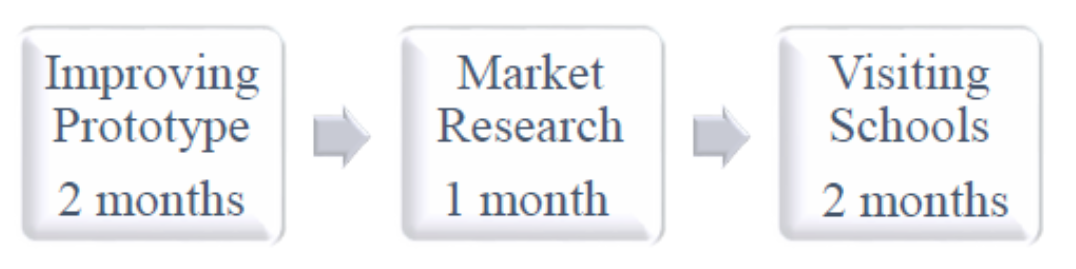
\includegraphics[width=0.7\textwidth]{education/STFCproposal/STFCProposal_Timeline2.png}
    \caption{A brief timeline of the planned project so far, once STFC funding has been granted}
    \label{fig:PropTimeline_STFC}
\end{figure} 
\end{center}

Figure \ref{fig:PropTimeline_STFC} shows how long each portion of the project will last. According to our initial plan, the project should last 5 months. After this period, we will evaluate feedback that we have collected from the schools and look for ways to carry out improvements.

\begin{enumerate}
\item \textbf{Perfecting Apparatus}

The apparatus that we have assembled as part of our group project is rather robust and not easily movable. It consists of the following parts: loudspeaker (woofer), rigid wooden plate, fold back clippers, wires with crocodile clip, amplifier power supply cable, synchronized function generator, BNC cables and 6.5'' petri dish. We have tried silicone oil as liquid in the petri dish, however, from our experience, water mixed with soap is a better and cheaper alternative.

We wish to improve this apparatus so that all parts can be contained by a compact wooden box. This will make the device easy to move and also look more professional. The device can also be used also with a smart phone serving as a function generator, which would enable some room for interaction with students. To achieve this, we have to make some small modifications to the set up. A schematic of a possible version of this apparatus can be seen in.  \ref{fig:apparatus_diagram_STFC}.

\begin{figure}
\centering
    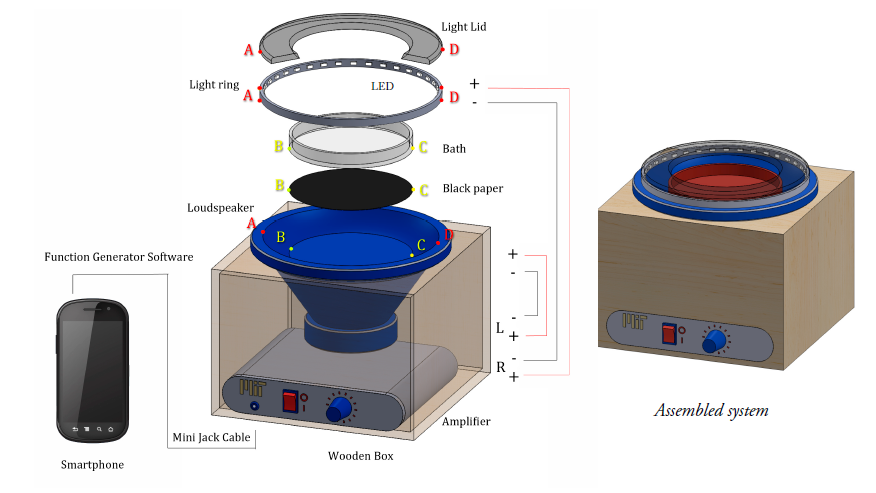
\includegraphics[width=16.14cm,height=9.647cm]{education/STFCproposal/Apparatus_STFC.png}
    \caption{Potential apparatus setup, post improvements and granting of STFC funding.}
    \label{fig:apparatus_diagram_STFC}
\end{figure}

We have also made simulations which demonstrate how quantum particles should behave according to pilot-wave theory. Due to the limited amount of time, these simulations are rather simple. However, in the future, these could be made into short films to show to students.

In addition, we have recorded footage of the bouncing droplets using an ultra-high speed camera. This enables the viewers to have an even more detailed look at these phenomena and really see what is happening step by step.


\item \textbf{Market Research}

We think that it is extremely important to properly investigate the potential this project has. This will firstly consist of determining the exact age-group that we wish to aim this project at and finding and contacting as many schools as possible to see if they are interested in hosting us as outreach speakers.

In order to have a significant impact on the long-term decisions that students make, it is crucial to find the adequate age-group that we mainly want to outreach to. If the students are too old, the impact on them is significantly smaller, on the other hand, if they are too young, they might not have the technical knowledge that is required to fully grasp the experiment. We hope to find the critical phase in the students' life when they are yet to decide how to continue their studies, but they are already aware of the existence of quantum mechanics.


\item \textbf{Outreach to Schools}

Using our prototype, we have visited a school already (Chesham Grammar school), as a trial for or long-term plan. From our experience, students found the apparatus to be eye-catching and innovative. We made preliminary feedback forms which were given to the students we presented to. The results are unanimous: 95\% of the students found the demonstration useful in understanding the quantum world, and more than 60\% of them were more interested in studying physics in the future after the demonstration. 

We are also planning to make a non-technical script which enables anyone to construct the device. This would include an equipment list, a building guide experiments and lesson plans that anyone can carry out using the device.

In addition to these, we also want to produce a short video in which we would explain the phenomena and demonstrate how to produce, manipulate and experiment with the bouncing droplets. \ 

\end{enumerate}

\subsection{Summary}

We will produce a compact apparatus which is easily movable and demonstrates quantum mechanical phenomenon using bouncing droplets. Then, we will contact schools, potentially with the help of STFC, to find possible platforms where we can demonstrate our project. We will ask the participating students and teachers for feedback and improve accordingly. 


\bigskip

\subsection{Project Personnel}

Steven Vuong and Kelvin Fang will be responsible for the improvement of the apparatus and its branding. Steven will make sure that the device is compact and easy to use and Kelvin will ensure that the apparatus is visually appealing. In addition, they will try to reduce the cost of the equipment as much as possible, thus making it more affordable. Furthermore, they will also seek external consultants (designers and engineers) to obtain expert opinions for further improvements.

Georges Ajaka and Alex Stock will further develop simulations of the quantum effects that can be visualised using the device. This job requires a high level of programming skills so, in the future, the help of an expert might be necessary. The simulation will hopefully enable the students to see similarities between the quantum world and bouncing droplets. We are planning to make the code they produce open-source.

The market research will be conducted by Chong Keat Gea and Benjamin Berczi. They will contact schools to gauge interest in this outreach opportunity. Then, surveys would be sent to the schools that are interested. These surveys will contain questions about what would interest the students and what they would prefer to see during a demonstration, along with the technical understanding of physics possessed by their average student. 

After conducting the market research, Johnny Allain-Labon and Mohit Motwani will visit schools that expressed interest and demonstrate our device in person. They will work alongside STFC associates to deliver an hour long demonstration. Johnny and Mohit have already prepared a guest lesson plan and an evaluation form for it as well, with the assistance of the Physics Department outreach officer, Dr. Mark Fuller. 

\subsection{Related Activities}

There are many papers about this phenomenon and there has been several attempts to use it as a tool for public engagement. However, we feel that its potential hasn't been fulfilled. Examples of papers published on this topic include:
\begin{enumerate}
    \item J. Walker. Drops of liquid can be made to float on the liquid. What enables them to do so? Sci. Am, 238(6):123--129, 1978
    \item Y. Couder, S. Proti\'ere, E. Fort, and A. Boudaoud. Dynamical phenomena: Walking and orbiting droplets. Nature, 437(7056):208--208, 2005.
    \item R. Brady, R. Anderson. Why bouncing droplets are a pretty good model of quantum mechanics \url{https://arxiv.org/abs/1401.4356}
\end{enumerate}

In terms of public engagement, attempts have been made using YouTube. The most viewed YouTube video on this topic is by Veritasium: ``Is This What Quantum Mechanics Looks Like?'', \url{https://www.youtube.com/watch?v=WIyTZDHuarQ\&t=185s}. 

Although this video demonstrates the similarities between the bouncing droplet phenomenon by referencing papers, it does not show how droplets are made and how they behave. In addition, it doesn't make efforts to explain the physics of it in detail for the younger groups of audience. 

\subsection{Awareness raising, dissemination and networking}

We hope to raise awareness by giving the public a closer look at modern science; by making quantum mechanics more visual. We hope to influence adults as well as students. The project's main aim is to have an impact on students, however, using social media, adults can be reached too. 

During the demonstrations in schools, students will get an insight of how quantum mechanics works and how it can be manipulated. 

In addition, we plan to upload our video, in which we demonstrate our project, to Youtube as well. Youtube provides us access to a widely used platform with which we can reach many people from different backgrounds.

Moreover, students will be able to network with us, university students, and also STFC associates to gain knowledge about their options in science. 

\subsection{Monitoring and Evaluation}

As mentioned before, we will use feedback forms and surveys to gain audience feedback. These forms will be processed and evaluated by the market research team. They will enable us to make improvements in order to make our product more relatable and exciting. 

YouTube provides us with immediate feedback as well, with which we can get an impression of the experience that people of all ages get. This will help improve the apparatus and presentation to a wider range of audiences. 


\subsection{Justification of Resources}
\bigskip
\begin{table}
\centering
\begin{tabular}{|c|c|c|c|}
\hline
\textbf{Category}& \textbf{Product} & \textbf{Cost(\pounds)} & \textbf{Source} \\
\hline
\multirow{10}{4em}{Apparatus} & Loudspeaker & \pounds25 & Amazon\\
& Amplifier (with power supply cable) & \pounds18 & Amazon \\ 
& 4" Petri dish & \pounds3 & Amazon\\
& LED strips & \pounds9 & Amazon\\
& Mini-Jack cable & \pounds6 & Amazon\\
& Glue and Paper & \pounds3 & Ryman\\
& Clippers & \pounds5 & Hardware store\\
& Wooden plate & \pounds3 & Hardware store\\
& Kitchen soap & \pounds2 & Tesco\\
& \textbf{Category Cost} & $ \pounds74 \times 10= \pounds 740$ &  \\
\hline
\multirow{3}{4em}{Camera} & Sony DSCRX100M4 & \pounds792 & Amazon\\
& 4'' Hama Star 61 Camera Tripod & \pounds3 & Amazon\\
& \textbf{Category Cost} & \pounds814 &  \\
\hline
\multirow{3}{4em}{Personnel} & Designer & \pounds1500 &  \\
& Engineer & \pounds1000 &  \\
& \textbf{Category Cost} & \pounds 2500 &  \\
\hline
\textbf{ }& \textbf{Grand Total} & \textbf{\pounds4054} &   \\
\hline

\end{tabular}
\caption{Details of the projected cost for developing the outreach project further, inluding section by section costs}
\label{table:STFC_costs}
\end{table}
\bigskip

The costs to build the prototype we have constructed part by part can be seen in \ref{table:STFC_costs}. It can be seen that it costs approximately {\pounds}74 to build our apparatus. From the wooden plate a wooden box can be constructed using laser printing -- which is available for us, UCL students at the Institute of Making. The kitchen soap mixed with water can replace the silicone oil in the experiment, which lowers the costs. 

In the first round of our plan, we want to visit and supply a minimum of 10 schools, in order to gain a sufficient amount of feedback for future improvements. This would mean 10*{\pounds}74={\pounds}740.

In addition, we require a high-speed camera to record excellent quality footage as explained before. We also need a camera stand which allows for the camera to be held steady.

Moreover, we plan to involve external personnel in the project: an engineer and a designer. We would employ them for about two weeks. The ratio of the average salary for a designer to an engineer is about 1:1.5. Therefore the salaries we offer have the same ratio.

In conclusion, we require {\pounds}4054 to conduct our project and reach schools in the UK, in order to improve public engagement regarding STEM stubjects.